\documentclass[12pt]{article}
\linespread{1.3}
%\usepackage{arev}
\usepackage[T1]{fontenc}
\usepackage[utf8]{inputenc}
\usepackage{polski}
\usepackage{geometry}
\usepackage{graphicx}
\usepackage{enumitem}
\usepackage{textcomp}
\usepackage{hyperref}
\usepackage{subcaption}
\usepackage{caption}
\usepackage{mdwlist}
\usepackage{lscape}
\newgeometry{tmargin=2cm, bmargin=2cm, lmargin=3cm, rmargin=3cm}
        
\begin{document}

%==================================================================================
% STRONA TYTUŁOWA
%----------------------------------------------------------------------------------
\begin{titlepage}
\center


%--------------  NAGŁÓWKI ---------------------------------------------------------

\textsc{\Large Politechnika Wrocławska}\\[0.5cm] % Name of your university/college
\textsc{\large Wydział Elektroniki}\\[5cm] % Major heading such as course name

%--------------  TYTUŁY   ---------------------------------------------------------

\textsc{\LARGE PROJEKT Z BAZ DANYCH}\\[2cm] % Minor heading such as course title
{ \Large \bfseries Dziennik szkolny}\\[5cm] % Title of your document
%--------------  TERMIN ZAJĘĆ -----------------------------------------------------
\begin{minipage}{0.83\textwidth}
\begin{flushleft} \large
Termin zajęć: Środa, 9-11 \\[2cm]
\end{flushleft}
\end{minipage}
\\[2cm]

%--------------  AUTORZY  ---------------------------------------------------------

\begin{minipage}{0.4\textwidth}
\begin{flushleft} \large
\emph{Autorzy:}\\
Adam \textsc{Mielniczek}\\
Michał \textsc{Kowalski}\\
Maciej \textsc{Pająk}\\
\end{flushleft}
\end{minipage}
~
\begin{minipage}{0.4\textwidth}
\begin{flushright} \large
\emph{Prowadzący zajęciar:} \\
dr inż. Roman \textsc{PTAK} 
\end{flushright}
\end{minipage}\\[2cm]

%--------------  DATA     ----------------------------------------------------------

{\large Wrocław, 2020}\\[1cm] % Date, change the \today to a set date if you want to be precise

\vfill 
\end{titlepage}
%^^^^=================================^^^^^===================================^^^^^^^^

%=====================================================================================
% SPIS TREŚCI
%-------------------------------------------------------------------------------------
%\tableofcontents
\newpage
%^^^^=================================^^^^^===================================^^^^^^^^



%=====================================================================================
% ROZDZIAŁ 1
%-------------------------------------------------------------------------------------
\section{Wstęp}
\subsection{Cel projektu}
\hspace{0.5cm} Celem projektu jest zapoznanie się z praktycznym użyciem (zaprojektowaniem oraz implementacją) narzędzia, jakim jest baza danych, zaznajomienie się z językiem SQL oraz poznanie sposobów na mądre przechowywanie i przeszukiwanie dużych zbiorów danych. Drugi cel to opracowanie aplikacji dostępowej, która będzie zapewniała dostęp do bazy danych osobom, nieposiadającym wiedzy z zakresu działania baz danych.

\subsection{Zakres projektu}
\hspace{0.5cm} Projekt składać będzie się z 5 etapów:
\begin{enumerate}
    \item Opis wymagań projektu,
    \item Schemat konceptualny, logiczny oraz fizyczny relacji,
    \item Implementacja bazy danych,
    \item Napisanie aplikacji dostępowej dla użytkowników,
    \item Prezentacja, testy i podsumowanie całości projektu.
\end{enumerate}

%^^^^=================================^^^^^===================================^^^^^^^^


%=====================================================================================
% ROZDZIAŁ 2
%-------------------------------------------------------------------------------------
\section{Opis wymagań}
%-------------------------------------------------------------------------------------
\subsection{Opis działania}
\hspace{0.5cm} Dziennik szkolny będzie zestawem bazy danych oraz aplikacji dostępowej, która umożliwi podstawowe zarządzanie szkołą. Docelowym klientem jest szkoła licealna średniej wielkości (około 400-500 uczniów). System ma spełniać podstawowe wymagania związane z funkcjonowaniem systemu nauczania w szkole takie jak np ocenianie i~sprawdznaie obecności uczniów na zajęciach.
%-------------------------------------------------------------------------------------
\subsection{Rodzaje kont użytkownika}

\hspace{0.5cm} Docelowy projekt będzie pozwalał na zalogowanie się na wymienione niżej rodzaje kont:
\begin{itemize*}
    \item Dyrektor (Administrator),
    \item Nauczyciel,
    \item Rodzic,
    \item Wychowawca,
    \item Uczeń,
    \item Kasa szkolna.
\end{itemize*}
%-------------------------------------------------------------------------------------
\subsection{Wymagania funkcjonalne}

\hspace{0.5cm} Funkcjonalności są kategorii CRUD, chyba że w nawiasie w danym punkcie podano inaczej.

\subsubsection{Administrator}
\begin{itemize*}
    \item Zarządzanie uczniami,
    \item Zarządzanie nauczycielami,
    \item Zarządzanie klasami,
    \item Zarządzanie kontami użytkowników,
    \item Wprowadzanie nagan dyrektorskich uczniom,
    \item Generowanie świadectwa dla ucznia na zakończenie roku szkolnego - eksport do~zewnętrznego pliku (C).
\end{itemize*}

\subsubsection{Nauczyciel}
\begin{itemize*}
    \item Wpisywanie tematu zajęć i sprawdzanie listy obecności,
    \item Podgląd obecności danego ucznia z danej klasy (R),
    \item Podgląd oraz wpisywanie uczniom ocen cząstkowych i ich wag,
    \item Wystawianie ocen semestralnych i końcowych (także możliwość ich edycji lub~usunięcia w razie przypadkowego wystawienia),
    \item Dodawanie terminów kartkówek, sprawdzianów itp. dla danej klasy,
    \item Wpisywanie uczniom uwag.

\end{itemize*}
\subsubsection{Wychowawca}
\begin{itemize*}
    \item Dostęp do terminarza klasy wychowawczej - wychowawca ma możliwość podglądu wszystkich form (sprawdzianów, kartkówek) zaplanowanych w terminarzu danej~klasy (R),
    \item Usprawiedliwianie nieobecności uczniów (U),
    \item Wystawianie ocen z zachowania, a także możliwość ich korekty lub usunięcia przy przypadkowym wpisaniu,
    \item Dostęp do statystyk każdego ucznia z klasy wychowawczej oraz całej klasy wychowawczej (R).
\end{itemize*}

\subsubsection{Uczeń}
\begin{itemize*}
    \item Przegląd otrzymanych ocen i obecności (R),
    \item Przegląd terminarza (R).
\end{itemize*}
\subsubsection{Rodzic}
\begin{itemize*}
    \item Przegląd otrzymanych ocen swojego dziecka (R),
    \item Przegląd dziennika uwag swojego dziecka (R),
    \item Przegląd nierozliczonych płatności (R),
    \item Usprawiedliwianie nieobecności swojego dziecka.
\end{itemize*}
\subsubsection{Kasa}
\begin{itemize*}
    \item Dodawanie nowej płatności do ucznia lub całej klasy,
    \item Zatwierdzanie płatności w systemie,
\end{itemize*}
%-------------------------------------------------------------------------------------
\subsection{Wymagania niefunkcjonalne}
%-------------------------------------------------------------------------------------
\subsubsection{Wykorzystywane technologie i narzędzia}
\begin{itemize*}
    \item Dostęp z poziomu systemów Linuxowych i Windowsa (możliwa aplikacja webowa),
    \item Interfejs graficzny,
    \item Baza danych zrobiona w systemie MariaDB.
\end{itemize*}
%-------------------------------------------------------------------------------------
\subsubsection{Rozmiar bazy danych}
\begin{itemize*}
    \item Baza danych powinna pozwalać na założenie około 400-500 kont Uczniów, 2 razy większą ilość kont rodziców oraz około 30 kont nauczycieli,
    \item Przewidujemy, że w każdym roku szkolnym będzie przechowywane około $60-120$ tys. ocen, około miliona obecności oraz około $30$ tys. tematów lekcyjnych.
    \item Prawdopodobnie w "godzinach szczytu" z dziennika korzystać będzie około $80$ osób.
\end{itemize*}
%-------------------------------------------------------------------------------------
\subsubsection{Bezpieczeństwo systemu bazodanowego}
\begin{itemize*}
    \item Logowanie się do systemu nazwą użytkownika i hasłem (hasło w bazie w postaci zaszyfrowanej),
    \item Możliwość zresetowania hasła na e-mail,
    \item Możliwość włączenia dwustopniowej weryfikacji (kod przysyłany na e-mail).
\end{itemize*}
%-------------------------------------------------------------------------------------
%\subsection{Przyjęte założenia projektowe}
%^^^^=================================^^^^^===================================^^^^^^^^

%=====================================================================================
% ROZDZIAŁ 3
%-------------------------------------------------------------------------------------
\section{Modele bazy danych}

\hspace{0.5cm} Poniżej przedstawione schematy systemu bazodanowego zostały zrobione w aplikacji webowej draw.io.

Przykładem normalizacji przeprowadzonym na poniższych modelach jest przeniesienie pól imię oraz nazwisko z relacji rodzic, uczeń i nauczyciel do relacji użytkownik. Adres został także rozdzielony na części oraz miejscowość i ulica przeniesione do dodatkowej relacji (podejrzewamy, że większość uczniów będzie z jednej miejscowości, a~spora część także będzie mieszkać przy tej samej ulicy). Relacja nauczyciel przedmiotu dodana została w celu pozbycia się relacji wiele do wielu między nauczycielem, a nauczanym przez niego przedmiotem. To samo dotyczy relacji opiekunowie, która ułatwia połączenie rodzica z uczniem.

Ze względów bezpieczeństwa hasło przechowywane w bazie danych będzie szyfrowane algorytmem MD5 - stąd długość zaszyfrowanego hasła - zawsze 32 znaki.

\begin{landscape}
\subsection{Model konceptualny}

\begin{figure}[h!]
    \centering
    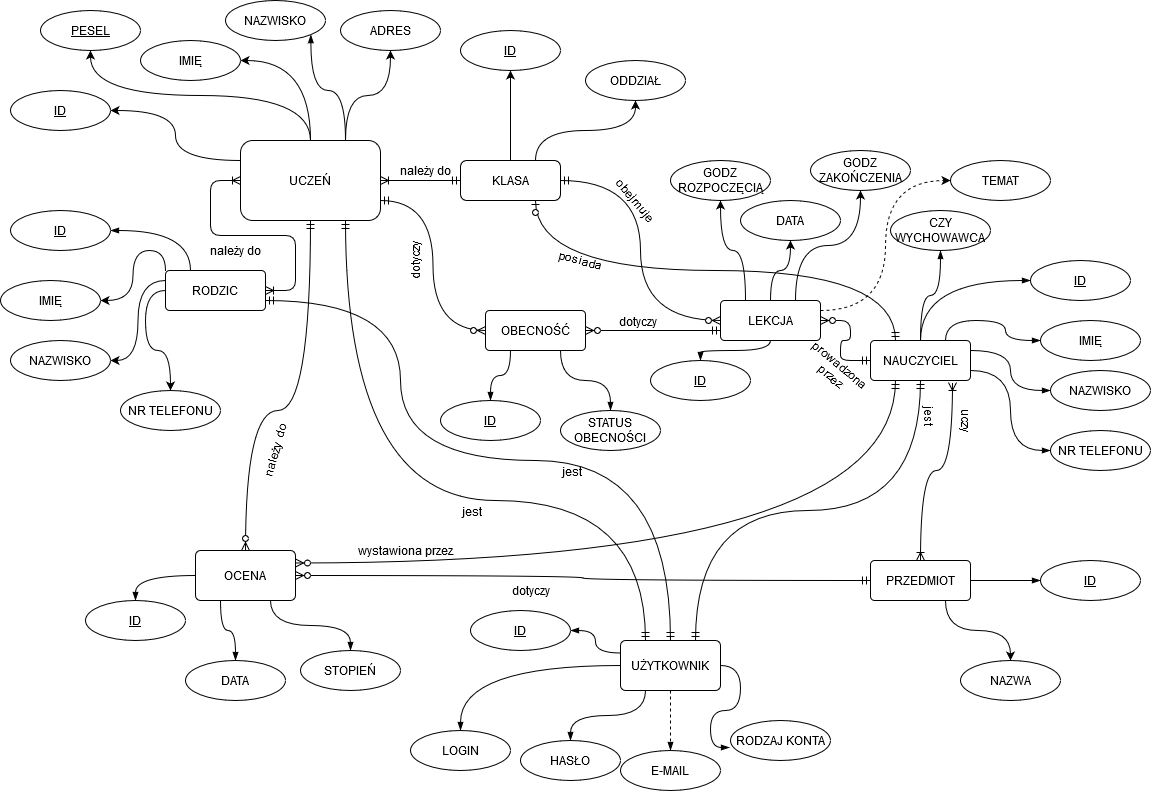
\includegraphics[scale=0.47]{MKonceptualny.png}
    \caption{Model konceptualny encji dziennika elektronicznego}
    \label{fig:mk}
\end{figure}

\newpage
\subsection{Model logiczny przed normalizacją}

\begin{figure}[h!]
    \centering
    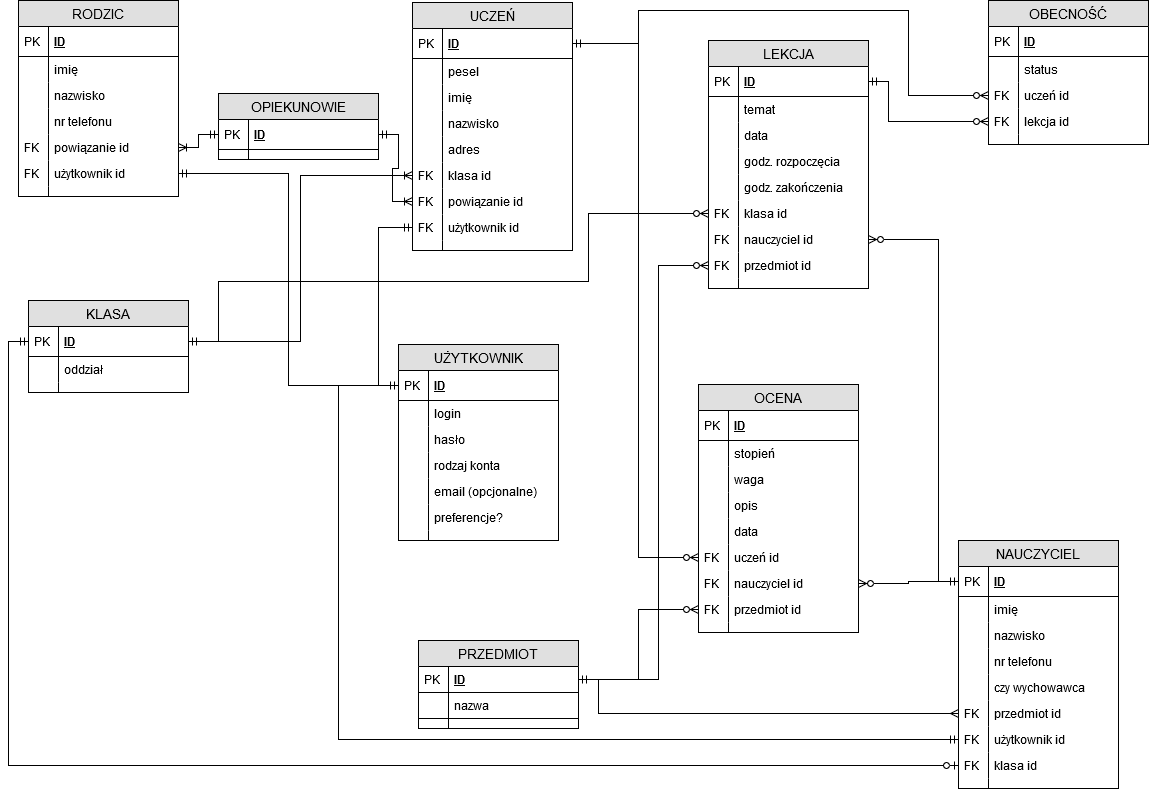
\includegraphics[scale=0.47]{MLogiczny.png}
    \caption{Model logiczny relacji dziennika elektronicznego}
    \label{fig:ml}
\end{figure}

\newpage
\subsection{Model fizyczny po normalizacji}

\begin{figure}[h!]
    \centering
    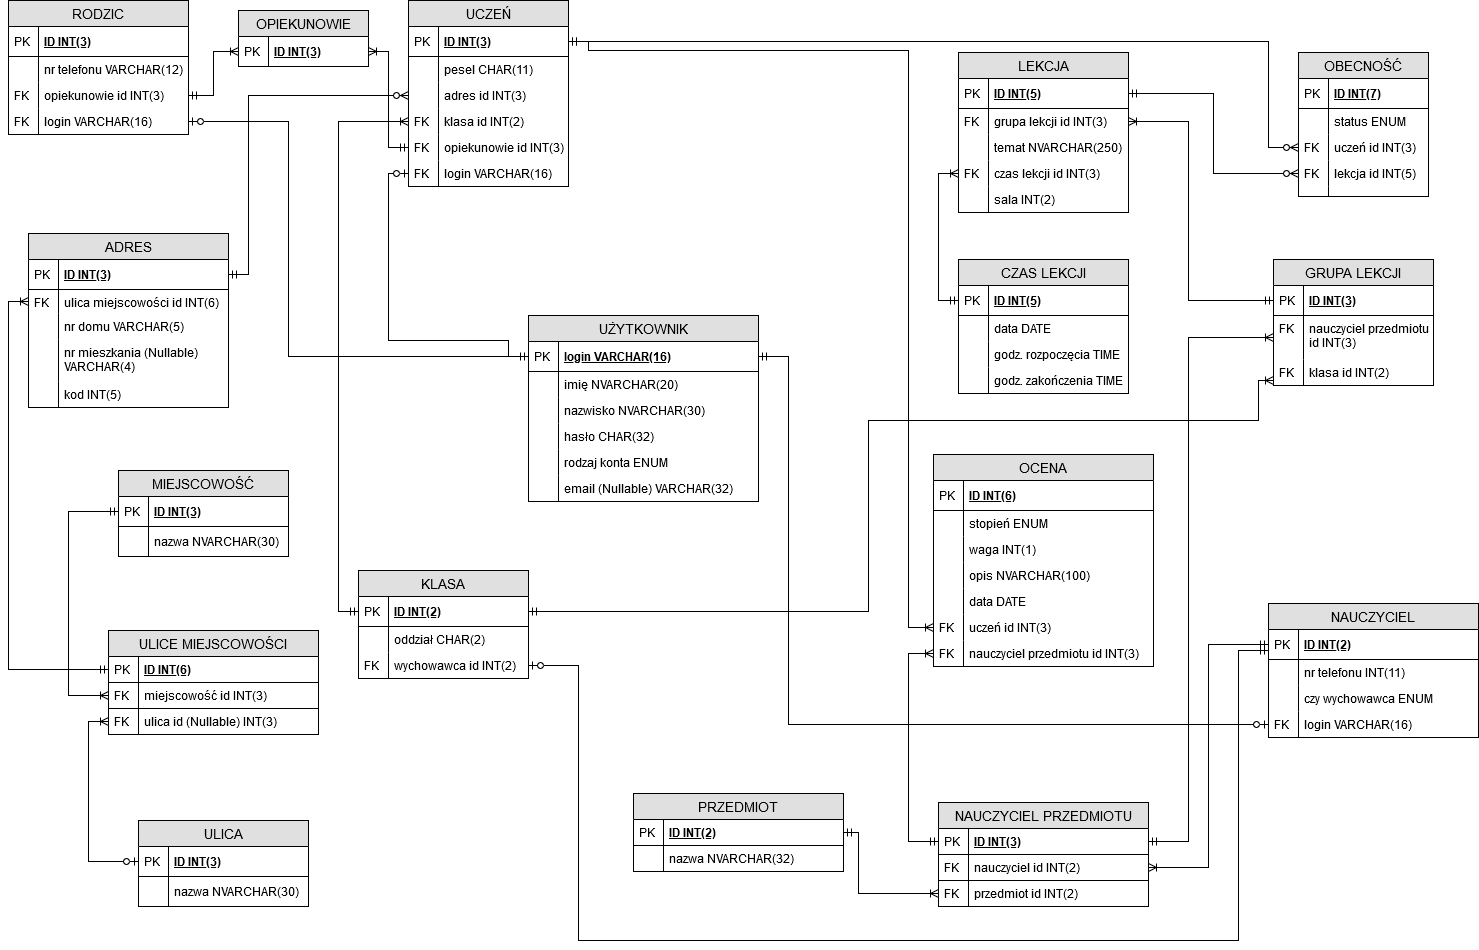
\includegraphics[scale=0.39]{MZnormalizowany.png}
    \caption{Model znormalizowany relacji dziennika elektronicznego}
    \label{fig:mf}
\end{figure}

\end{landscape}
\clearpage

\subsubsection{Model fizyczny i ograniczenia integralności danych}

\subsubsection{Inne elementy schematu - mechanizmy przetwarzania danych}
\subsubsection{Projekt mechanizmów bezpieczeństwa na poziomie bazy danych}
\subsection{Projekt aplikacji użytkownika}
\subsubsection{Architektura aplikacji i diagramy projektowe}
\subsubsection{Interfejs graficzny i struktura menu}
\subsubsection{Projekt wybranych funkcji systemu}
\subsubsection{Metoda podłączania do bazy danych - integracja z bazą danych}
\subsubsection{Projekt zabezpieczeń na poziomie aplikacji}
%^^^^=================================^^^^^===================================^^^^^^^^

%=====================================================================================
% ROZDZIAŁ 4
%-------------------------------------------------------------------------------------
\section{Implementacja systemu baz danych}
\subsection{Tworzenie tabel i definiowanie ograniczeń}
\subsection{Implementacja mechanizmów przetwarzania danych}
\subsection{Implementacja uprawnień i innych zabezpieczeń}
\subsection{Testowanie bazy danych na przykładowych danych}
%^^^^=================================^^^^^===================================^^^^^^^^


%=====================================================================================
% ROZDZIAŁ 5
%-------------------------------------------------------------------------------------
\section{Implementacja i testy aplikacji}
\subsection{Instalacja i konfigurowanie systemu}
\subsection{Instrukcja użytkowania aplikacji}
\subsection{Testowanie opracowanych funkcji systemu}
\subsection{Omówienie wybranych rozwiązań programistycznych}
\subsubsection{Implementacja interfejsu dostępu do bazy danych}
\subsubsection{Implementacja wybranych funkcjonalności systemu}
\subsubsection{Implementacja mechanizmów bezpieczeństwa}
%^^^^=================================^^^^^===================================^^^^^^^^


%=====================================================================================
% ROZDZIAŁ 6
%-------------------------------------------------------------------------------------
\section{Podsumowanie i wnioski}
%^^^^=================================^^^^^===================================^^^^^^^^


%=====================================================================================
% LITERATURA
%-------------------------------------------------------------------------------------
\section{Literatura}
%^^^^=================================^^^^^===================================^^^^^^^^



%=====================================================================================
% SPIS RYSUNKÓW
%-------------------------------------------------------------------------------------
\section{Spis rysunków}
%^^^^=================================^^^^^===================================^^^^^^^^


%=====================================================================================
% SPIS TABEL
%-------------------------------------------------------------------------------------
\section{Spis tabel}
%^^^^=================================^^^^^===================================^^^^^^^^

\end{document}
